% !TeX root = ../main.tex

\chapter{性能评估}
\label{chap:eval}

本章将对本系统的运行性能进行评估。
其中,\autoref{sec:eval-iso-rw}和\autoref{sec:eval-ssd-array}分别评估无读写干扰的SSD设计在单块和多块SSD上的效果;
\autoref{sec:eval-sla-enforcement}评估基于SLA曲线的IO请求调度的多租户性能隔离效果;
\autoref{sec:eval-sla-placement}是一个综合实验,通过模拟上百个具有不同存储需求的租户在云系统上获取资源,
展示了本系统的数据分布算法和无读写干扰的SSD阵列对系统中存储资源利用率的改善作用。

本章的实验均是在一个具有32核的Intel Xeon CPU E5-2698服务器上运行的,服务器的内存大小为192GB。
服务器上运行了Linux系统,内核版本为4.17.12。
系统实现基于的SPDK版本为19.04。
本实验中使用的SSD型号均为Samsung PM963,服务器与SSD之间互联为PCIe Gen3 x 4.

下文的\autoref{sec:eval-iso-rw}和\autoref{sec:eval-ssd-array}将会展示SLA曲线。
该SLA曲线中每个点的测量方法如下:
固定写吞吐,从小到大不断增大读吞吐,记录能使写吞吐保持在该固定值的最大读吞吐。
本章的实验中运行的写请求均为4KB顺序写,读请求均为4KB随机读。
实验中提到的“尾延迟”均为读请求的尾延迟。

\section{分离的读写时间窗口在单块SSD上的性能}
\label{sec:eval-iso-rw}

本节从尾延迟和吞吐两方面展示分离的读写时间窗口在单块SSD上的性能。
\autoref{fig:eval-iso-wr-latency}展示了在读吞吐为240KIOPS,写吞吐为80KIOPS,读写窗口时长比例为3:1时,
不同的读写时间窗口大小对读请求尾延迟的改善作用,并与无分离读写窗口的读写混合情况进行了比较。
该实验中的纯读情况是在读吞吐为240KIOPS,写吞吐为0,读写窗口比例不变的情况下测得的。
\autoref{fig:eval-iso-wr-thru}展示了分离的读写时间窗口对SSD带宽的提高作用。
在该实验中,读写窗口总时长被固定为200ms,将写窗口在总时长中的比例从$\frac{1}{10}$逐步提高到$\frac{9}{10}$,
并分别记录其SLA曲线,最终的曲线取所有曲线的最大值。

\begin{figure}[h]
  \centering
  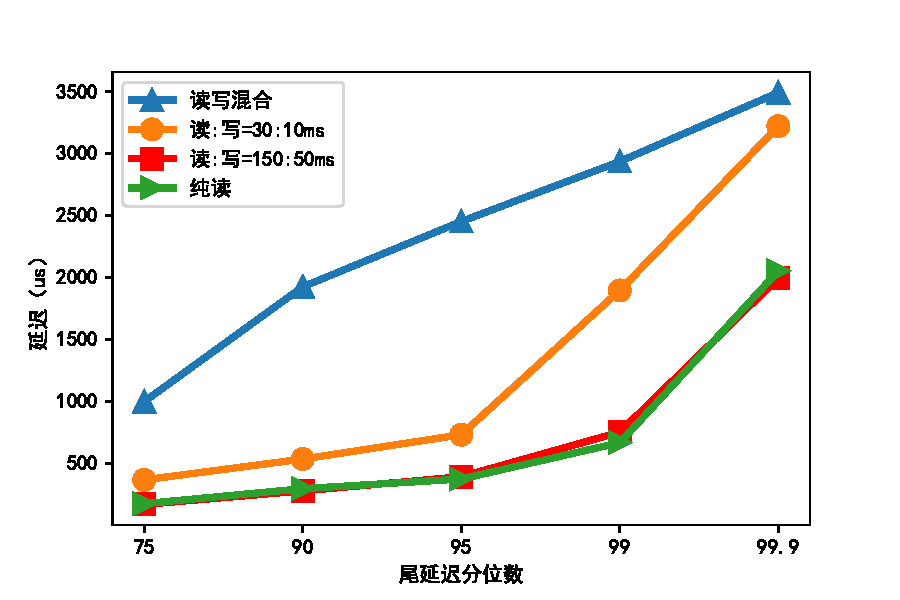
\includegraphics[width=0.8\textwidth]{thesis-iso-wr-latency.pdf}
  \caption{
        使用分离的读写时间窗口对单块SSD的尾延迟。
      }
  \label{fig:eval-iso-wr-latency}
\end{figure}

如\autoref{fig:eval-iso-wr-latency}所示,不同的读写时间窗口大小相比于完全读写混合的SSD都有对尾延迟的改善作用。
其中,30:10ms和150:50ms的读写时间窗口都可以将P95尾延迟降低至读写混合时的1/3至1/4。
相比之下,如\autoref{chap:impl}中的分析所述,较大的读写时间窗口对尾延迟的改善更大,150:50ms的读写时间窗口可以将尾延迟降低到与纯写几乎一致的水平。
这是因为较大的读写时间窗口避免了过多的读写窗口切换。


\autoref{fig:eval-iso-wr-thru}展示了当使用最优的读写窗口时长比例时,SSD 的读写带宽将被大大
提高。特别地,当写窗口时长占总长度的4/10时(写吞吐100KIOPS至130KIOPS
的区间),读带宽提高到了不使用分离的读写窗口的 2 倍左右。这是由于使用分
离的读写时间窗口时,在读窗口不再有写请求的干扰,读请求的执行速度提高,
从而使得固定的写吞吐下读带宽大大提高。这使得 SSD 的 SLA 曲线接近线性,
即读带宽和写带宽分别与他们的时间窗口大小成正比。该图测得的 SLA 曲线是
阶梯状的,这是由于写窗口的时长比例是阶梯状变化的,如果进行更细粒度的调
节,将能得到更好的曲线。

\begin{figure}[h]
  \centering
  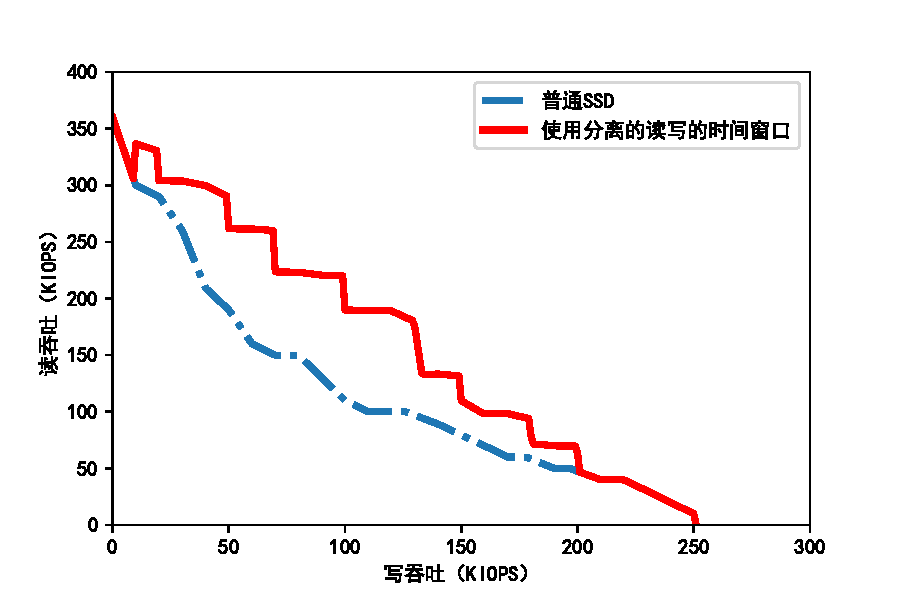
\includegraphics[width=0.8\textwidth]{thesis-iso-wr-thru.pdf}
  \caption{
        使用分离的读写时间窗口对单块SSD的带宽提升。
      }
  \label{fig:eval-iso-wr-thru}
\end{figure}


\section{无读写干扰的SSD阵列性能}
\label{sec:eval-ssd-array}

本节展示利用具有分离时间窗口的SSD组成无读写干扰的SSD的性能。
本节利用4台SSD组成阵列,它们的配置分别如下:
RAID-0为不利用任何冗余的有读写干扰的SSD阵列,被用作测试的基准;
RAID-10是分别利用两台SSD组成了RAID-1,并用两个RAID-1组成了RAID-0,
两个RAID-1的读写窗口时长均为100ms;
RAID-4是利用3台SSD作为数据盘,1台SSD作为冗余盘组成的,
数据盘的读窗口和写窗口时长分别为33ms和167ms,冗余盘分别为100ms和100ms。

\begin{figure}[h]
  \centering
  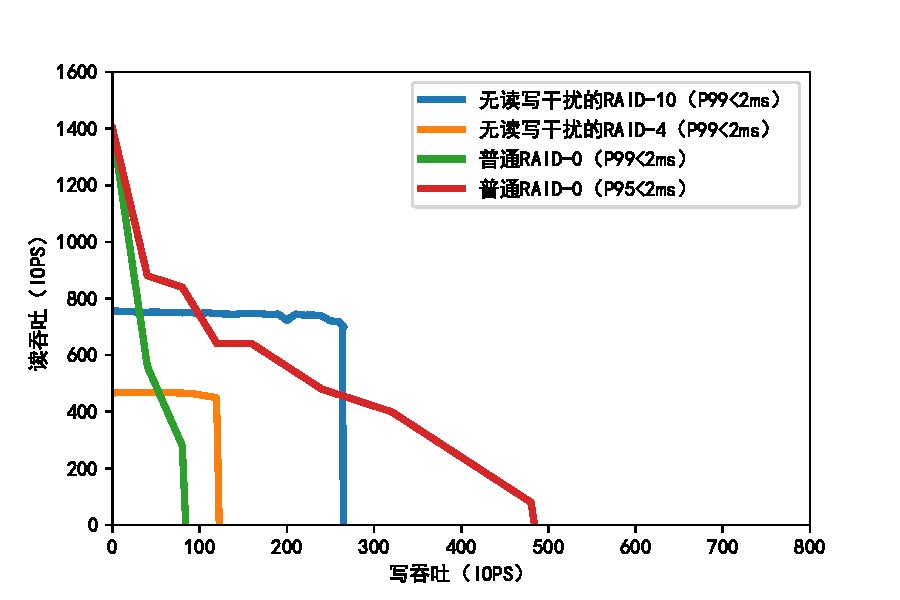
\includegraphics[width=0.8\textwidth]{thesis-eval-ssd-array.pdf}
  \caption{
        无读写干扰的SSD阵列的SLA曲线
      }
  \label{fig:eval-ssd-array}
\end{figure}

\autoref{fig:eval-ssd-array}截取了在P99尾延迟小于2ms的情况下,不同配置的SLA曲线。
由于RAID-10和RAID-4都采用了无读写干扰的技术,所以它们的SLA曲线接近方形。
相比之下,由于RAID-0受到读写干扰的影响,极小的写吞吐也会使得读延迟无法满足尾延迟的要求。
图中进一步将RAID-0的尾延迟要求放宽至P95小于2ms,在这种情况下,当读写吞吐都较大时,使用RAID-1仍能得到比RAID-0更好的吞吐。

图中的RAID-4拥有更多的数据盘,但是其能达到的最大带宽却远不如RAID-10,这是由于其具有的读写放大问题造成的。
首先,由于需要同时修改数据盘和冗余盘,RAID-4对于数据的一次更新需要两次读和两次写访问,这样的写放大对带宽造成了浪费。
其次,当一块数据盘处于写窗口中时,对该盘的读访问将由其它盘的数据恢复得出,需要$N - 1$次读访问,这样的读放大又影响了读带宽。

\section{基于SLA曲线的多租户性能隔离效果}
\label{sec:eval-sla-enforcement}

本节展示本系统基于SLA曲线限制共享同一物理资源的多个租户的访问带宽,并由此达到租户的尾延迟要求的能力。
为此,本节设计了以下两个类型的租户。

租户A是一个对访问速度要求较高的租户(例如在线数据库服务),因此他要求P95尾延迟小于2ms。
同时,它对存储资源的访问模式遵循一条直线,其最大读吞吐为120KIOPS,最大写吞吐为60KIOPS。
租户A的访问模式比较稳定,几乎任一时刻的吞吐都在SLA曲线之上或以下。
相比之下,与租户A共享同一块存储单元的租户B是一个“吵闹的邻居”。
他大多数时间占用的带宽不大,遵循的是最大读吞吐为70KIOPS,最大写吞吐为35KIOPS的曲线。
但是他会偶然将带宽提高到正常情况下的3倍,例如它开始进行大块的文件写操作。

本实验将两个租户在同一块SSD上运行60s,他们的吞吐均按上一段描述的规律随机变化。
\autoref{fig:eval-sla-enforcement}和\autoref{fig:eval-sla-enforcement-tail}将分别展示基于SLA曲线的请求调度对租户带宽和尾延迟的作用。

\begin{figure}[h]
  \centering
  \begin{subfigure}[b]{0.48\textwidth}
    \centering
    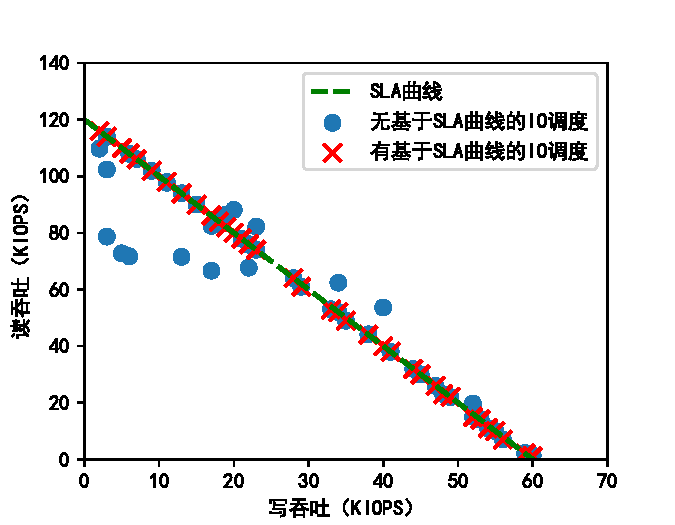
\includegraphics[width=\textwidth]{thesis-sla-enforcement-1.pdf}
    \caption{对尾延迟有高要求的租户A}
    \label{fig:eval-sla-enforcement-a}
  \end{subfigure}
  % \hfill
  \begin{subfigure}[b]{0.48\textwidth}
    \centering
    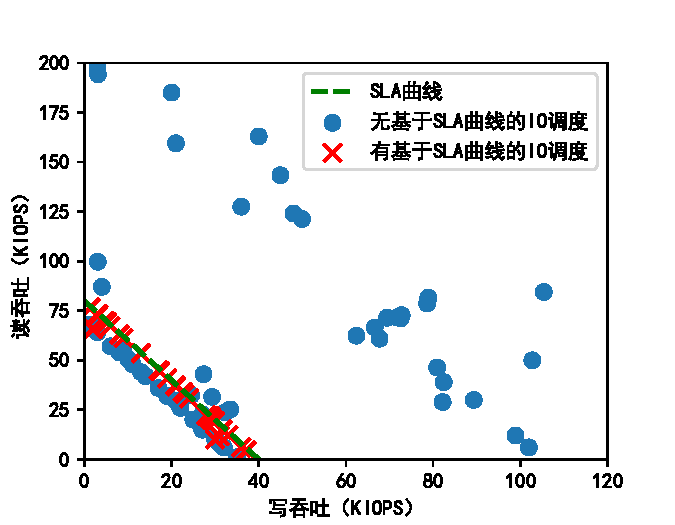
\includegraphics[width=\textwidth]{thesis-sla-enforcement-2.pdf}
    \caption{“吵闹的邻居”租户B}
    \label{fig:eval-sla-enforcement-b}
  \end{subfigure}
  \caption{基于SLA曲线的请求调度对租户带宽的限制作用}
  \label{fig:eval-sla-enforcement}
\end{figure}

如\autoref{fig:eval-sla-enforcement}所示,在不对租户进行基于SLA曲线的带宽限制时,租户B吞吐的异常增大将会导致
租户A的带宽受到异常的影响(如图中蓝色圆圈所示)。
此外,如\autoref{fig:eval-sla-enforcement-tail}所示,租户A的P95尾延迟也受到租户B的影响,多次超过其SLA要求。

因此,考虑给租户A和B按照其SLA曲线进行资源调度。
为避免影响租户B的整体带宽,分配给其的SLA曲线略大于其正常运行时的SLA曲线,使其异常变大的吞吐可以匀速通过。
如\autoref{fig:eval-sla-enforcement}所示,使用基于SLA曲线的调度后,两个租户的IO请求均稳定运行在其SLA曲线之下。
如\autoref{fig:eval-sla-enforcement-tail}所示,租户A的P95尾延迟也始终处于其尾延迟要求之下。
这是由于基于SLA曲线的请求调度可以始终保证整台SSD的读写吞吐位于其SLA曲线之下,从而保证理想的尾延迟。

\begin{figure}[h]
  \centering
  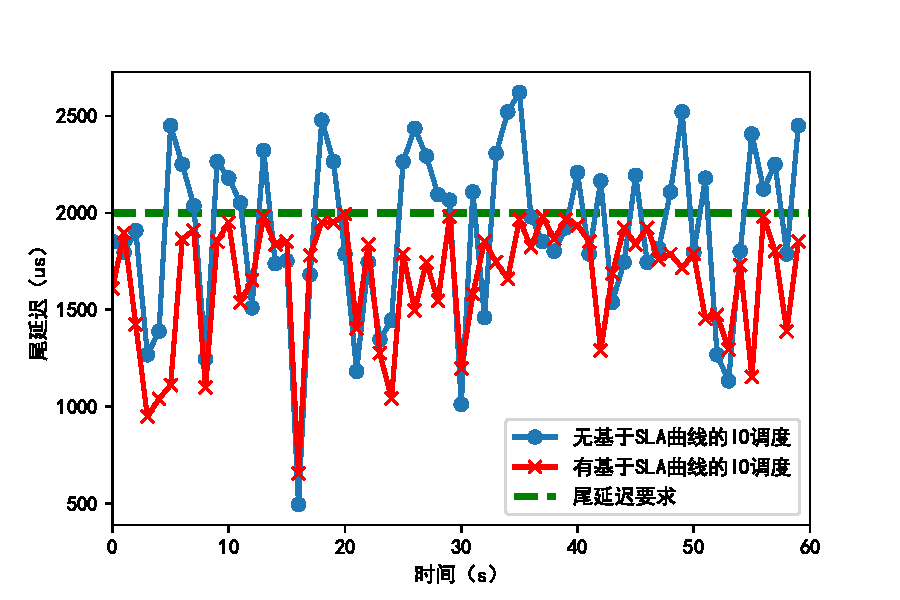
\includegraphics[width=0.8\textwidth]{thesis-sla-enforcement-tail.pdf}
  \caption{
        租户A的P95尾延迟。
      }
  \label{fig:eval-sla-enforcement-tail}
\end{figure}

\section{综合使用本文技术的资源效率提升}
\label{sec:eval-sla-placement}

本节利用一个大规模的租户部署情况展示综合利用无读写干扰的SSD阵列和基于SLA曲线的数据分布算法的存储系统的资源利用率。

为了在大量租户上进行实验,本实验采用软件模拟测试了上百个有SLA要求的租户在本系统中的资源分配情况。
由\autoref{sec:eval-sla-enforcement}所示,只要完成了数据分布,基于SLA曲线的运行时带宽调度就可以确保每个租户都满足其SLA。
具体来讲,本实验生成了三组租户,每组150个,其中对P90、P95和P99尾延迟有要求的租户各50个。
他们对存储空间的需求分别在[1, 30],[1, 100]和[1, 400]之间。
每一组中,每个租户对每个块的最大读带宽要求在[10, 80]之间,最大写带宽要求在[10, 30]之间。
每个租户的SLA曲线可能是1次、3次或5次曲线。
以上所有可能的选择均是通过均匀分布随机产生的。

本实验的模拟器根据以上租户需求,按照\autoref{chap:design}中提出的启发式数据分布算法选择合适的存储单元类型。
本实验中用到的存储单元类型除了\autoref{sec:eval-ssd-array}中提到的RAID-0、RAID-10和RAID-4外,还增加了由
3台SSD组成的RAID-1,它在任一时刻有一台SSD在进行读操作,有两台SSD在进行写操作,具有较好的读带宽。

\begin{figure}[h]
  \centering
  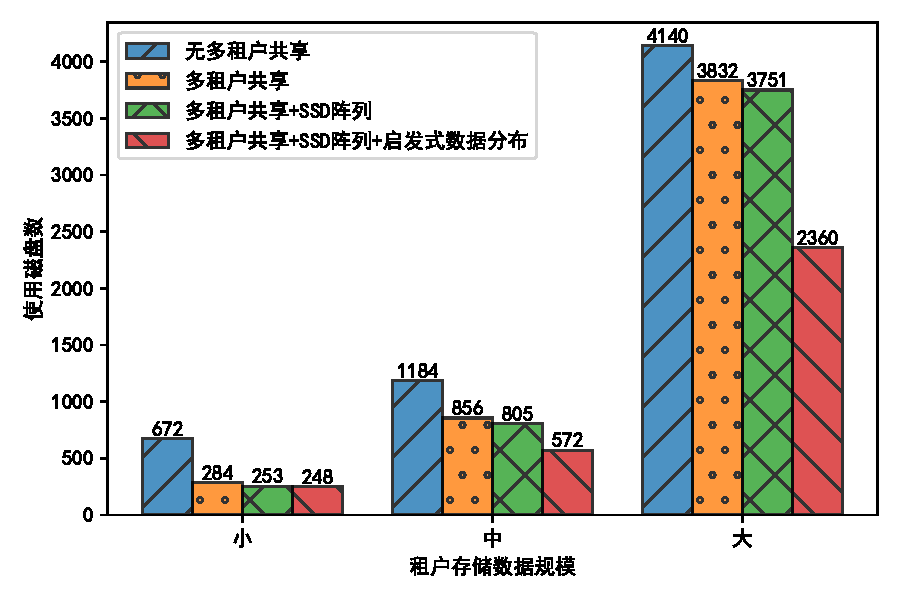
\includegraphics[width=0.8\textwidth]{thesis-sharing-savings.pdf}
  \caption{
        利用本系统提出的算法节约的SSD资源。
      }
  \label{fig:eval-sharing-savings}
\end{figure}

本实验共测试了以下情况。
“无多租户共享”指的是完全没有任何共享、每个租户都独自占有自己的存储资源的情况;
“多租户共享”指的是多个租户只要SLA曲线不冲突就可以共享同一块存储单元的情况;
“SSD阵列”指的是加入无读写干扰的SSD阵列,这些存储单元适合对尾延迟要求较高的租户;
“启发式数据分布”指的是多个租户共享同一块存储单元时,除了SLA曲线不能冲突,还根据数据分布算法选择最优的存储单元。

\autoref{fig:eval-sharing-savings}展示了满足所有租户的SLA要求所需的SSD个数。
在三个不同的数据集上,本系统提出的技术均可节约50\%左右的磁盘。
此外,当用户对存储资源的空间和带宽需求较小时,简单地让多个租户在满足SLA曲线的情况下共享同一个磁盘就可以大大节约磁盘。
在存储数据规模较小的数据集上,多租户共享就让总体使用的磁盘数下降了一半以上。
但是,当用户的存储数据较多时,简单地多租户共享的效果就不再明显。
在这种情况下,针对每个租户的SLA要求,选择合适的存储单元类型对总体磁盘使用数的影响就变得更大。

% Optional:用RocksDB跑一下,可以直接用db_bench?